\section{Hardware and Software platform}

In order to test the embedded implementation of MPC on real aircraft, one has to either use an existing platform or develop its own. Creating a custom hardware is a tedious job, but it is an investment that may eventually repay itself by providing complete control over platform's parameters and design. The key decision has been done to improve the existing design of custom control board (see \citep{baca2013} for more details) emphasizing possibility to reuse the code that has been already developed. A new version has been designed by incorporating experiences and observations from prior development. Following chapter firstly describes the UAV used for experimental validation of the control design, then there is new control board presented with overview of its features and capabilities, and lastly the software structure is discussed including used realtime operating system and custom matrix library.

\subsection{UAV platform}

The UAV is a custom built tricopter (fig. \ref{fig:tricopter}) with one propeller mounted on a tilting mechanism. It has a capability to pitch, roll and yaw just as any other multirotor UAV. The yaw control is supplied by the tilting mechanism while pitch and roll can be controlled by changing the ratio between rotational speed of all motors. All propellers are mounted directly on brushless motors, each one of them controlled by an individual ESC (electronic speed controller). It it capable of lifting payload of $150 \jed{g}$ while its weight is $450\jed{g}$. Its flight time is 7 minutes on average. Propellers are $5\times3.8 \jed{inch}$ in dimensions, mounted on motors by rubber bands to increase safety.

The aircraft is equipped with the \textit{KK2} board which provides the basic stabilization of pitch and roll angles ($\theta$, $\psi$) and yaw rate ($\dot{\phi}$). It is a low-cost ($\approx 30\jed{USD}$) commercial product with open-source software. It utilizes 3-axis MEMS gyroscopes and accelerometers to estimate $\theta$, $\psi$, $\dot{\phi}$ and allow the vehicle to be controlled as an RC model. It incorporates a set of nested PID controllers for both attitude axis. They can be easily using integrated display and buttons. It can handle various types of multirotor aircraft. Another important module is the \textit{px4flow} which is the only sensor used for localization (see section \ref{cap:px4flow} for more information).

\subsection{px4flow sensor}
\label{cap:px4flow}

The vehicle is localized in space by \textit{px4flow} sensor \citep{px4flow} (fig. \ref{fig:px4flow}), developed and produced by PixHawk \citep{pixhawk}. It integrates two sensors --- a camera for computing an optical flow and an ultrasonic rangefinder for measuring a distance from the ground. It provides an information about its velocity relative to the ground computed by the correlation of two consecutive images from the camera (the same principle as with most computer mice). The velocity is internally compensated from rotational motion by integrated gyroscope and finally scaled to absolute values using the altitude measured by the ultrasonic sensor. The sensor is able to measure velocities up to $0.5\jed{ms^{-1}}$ when flying in 1 meter altitude in good light conditions. The altitude is measured from $0.3\jed{m}$ to $4\jed{m}$. Data are sent in frequency around $70\jed{Hz}$ over UART (universal asynchronous receiver-transmitter) using MAVLink protocol.

\begin{figure}[tbp]
\centering

\begin{subfigure}[b]{0.55\textwidth}
	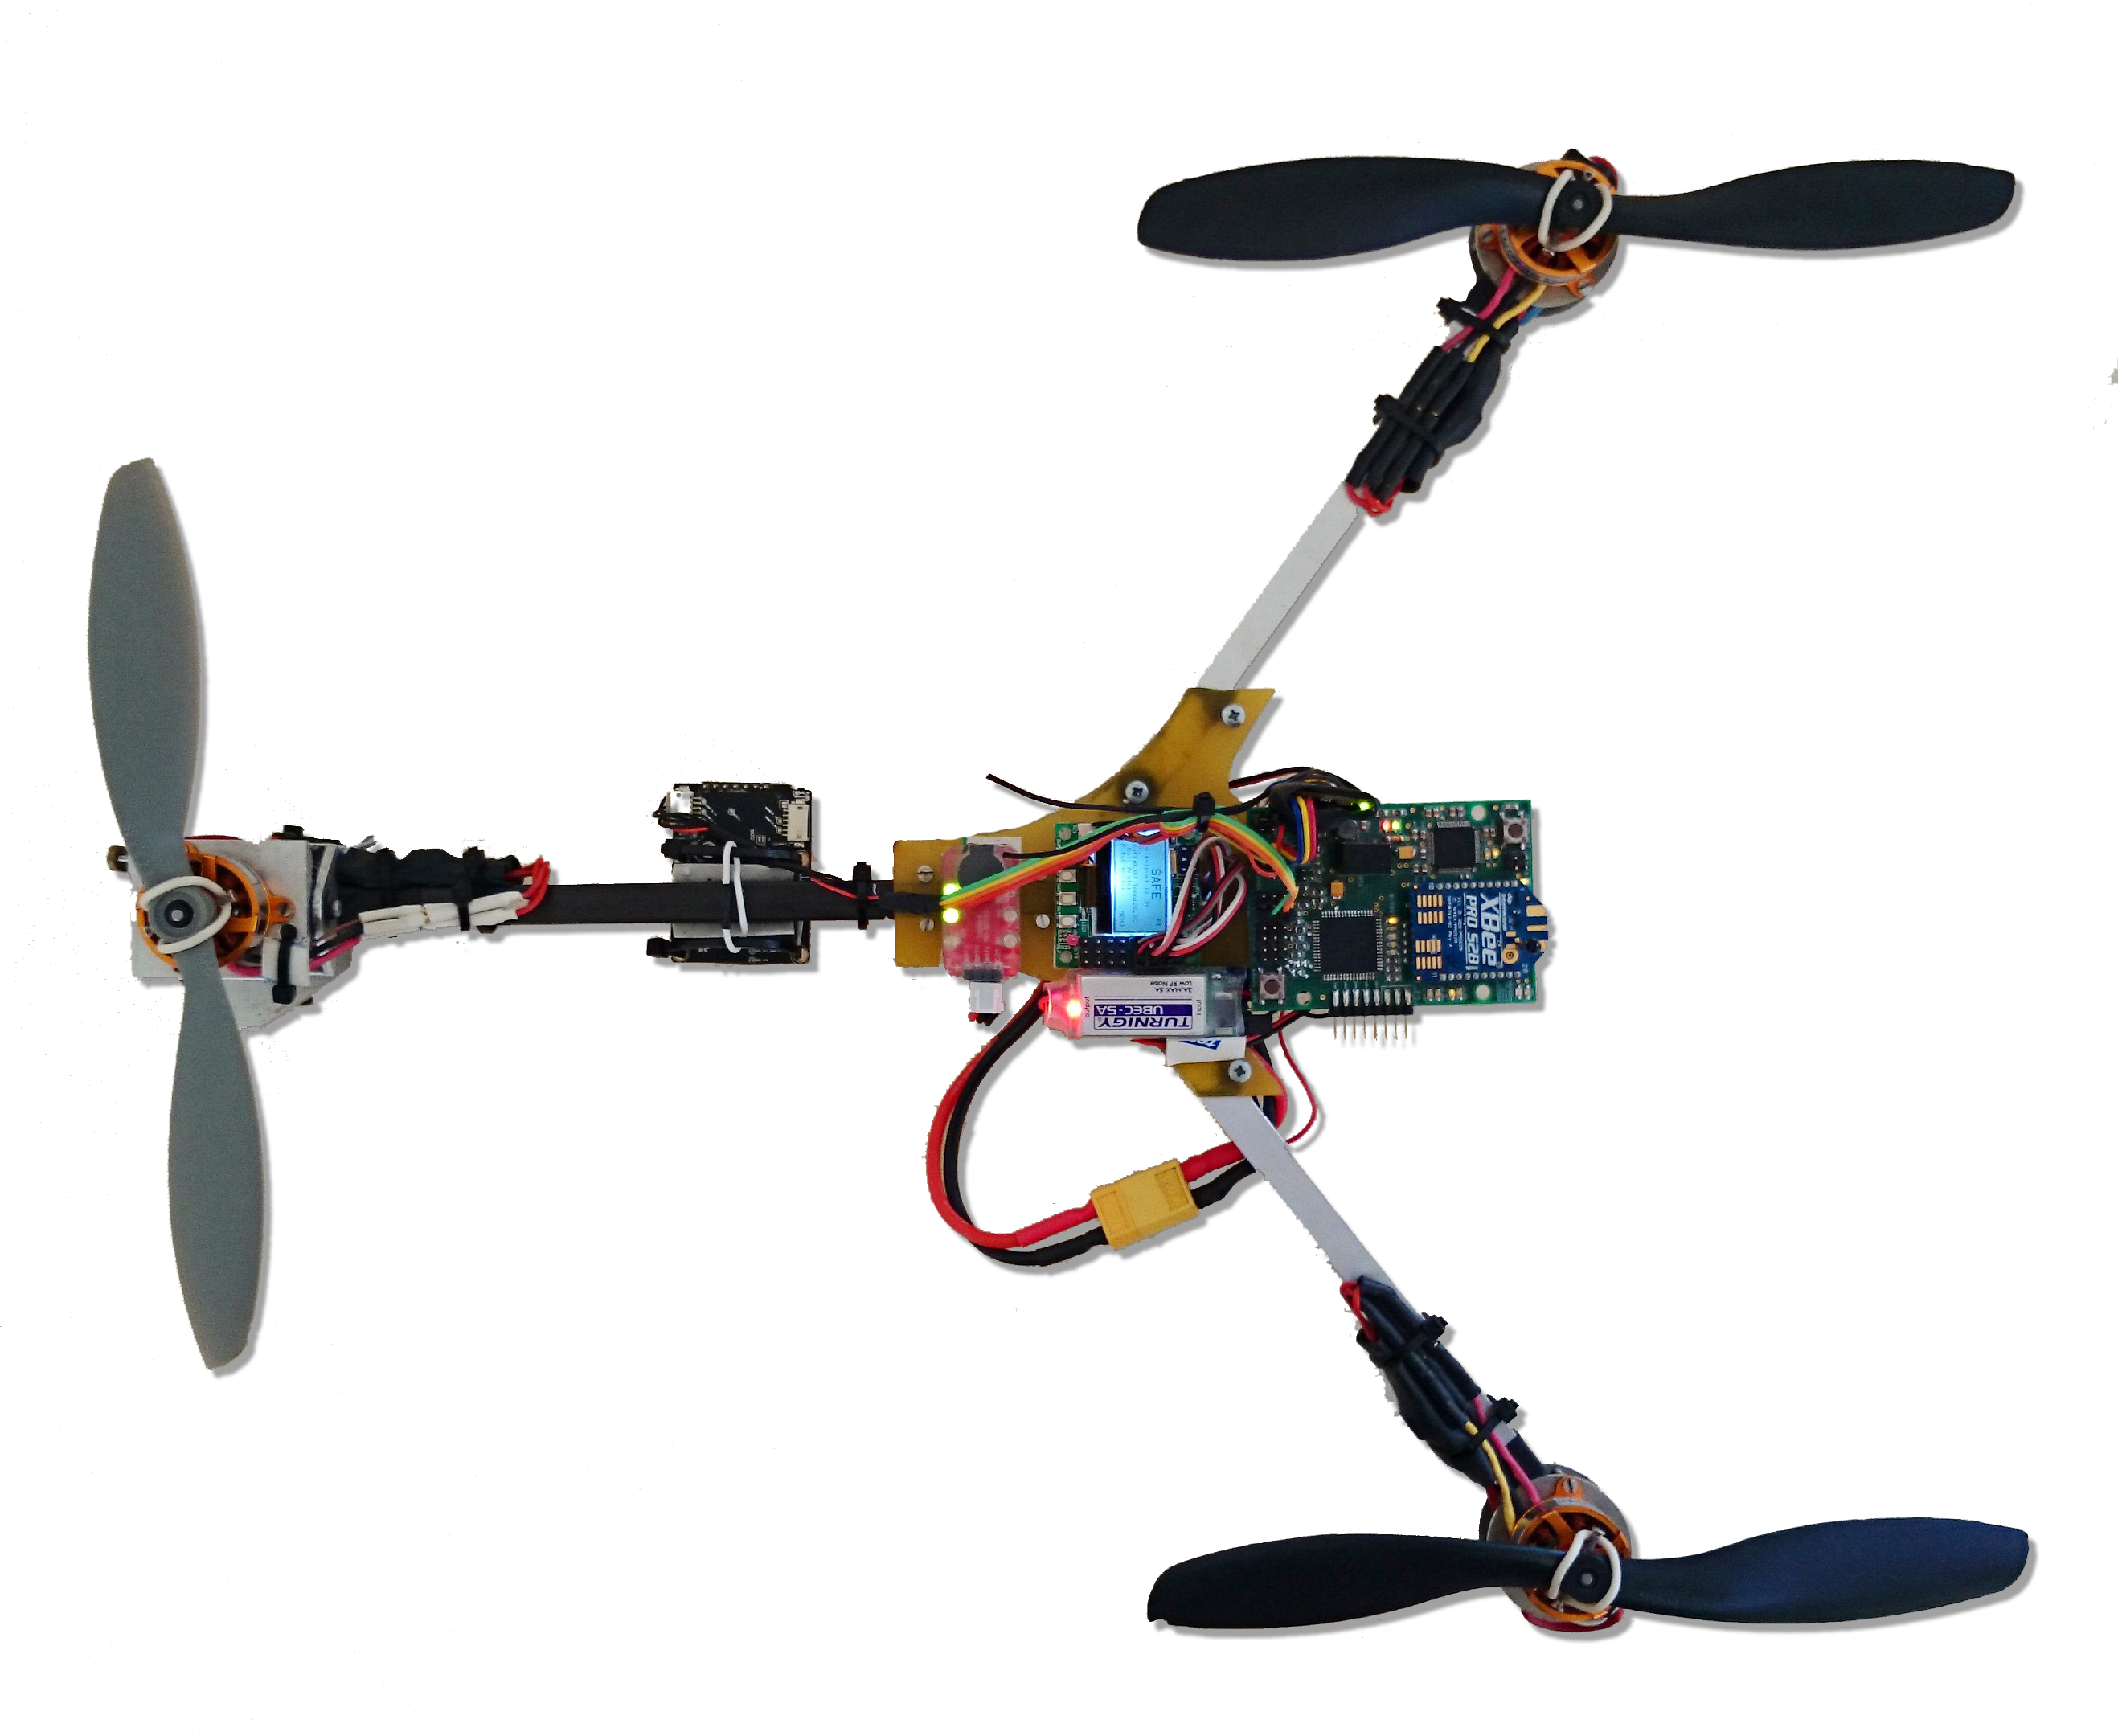
\includegraphics[width=\textwidth]{fig/tri1.jpg}
	\caption{Tricopter aircraft.}
	\label{fig:tricopter}
\end{subfigure}%
\begin{subfigure}[b]{0.45\textwidth}
	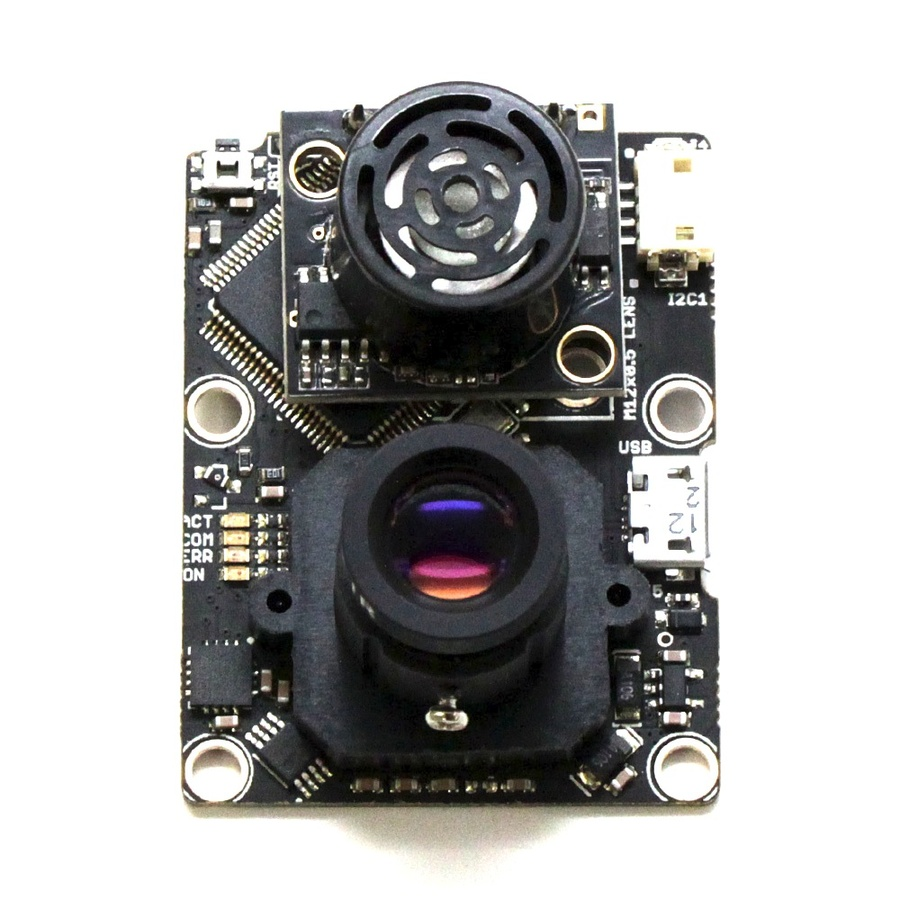
\includegraphics[width=\textwidth]{fig/px4flow.jpg}
	\caption{The px4flow sensor.}
	\label{fig:px4flow}
\end{subfigure}

\caption{Tricopter platform with px4flow optical flow sensor.}
\label{fig:tricopter_px4flow}
\end{figure}

\subsection{Custom control board v.2}

The control board v.2 is a significant improvement since the first version \citep{baca2013} which comprised only of a single 8-bit Atmel $\mu$-controller. After 1 year of using the old one, following needs emerged that started a development of the second version. The platform should support variety of connections for external sensors and modules, mainly via UART and $\mathrm{i}^2\mathrm{c}$. It should support onboard data logging which is necessary for debugging and capturing data for system identification. Another requirement is a presence of a telemetry module. The UAV should be able to send short packets of data to another helicopter and to the ground station (laptop). The main motivation is to allow simple telemetry data being displayed on laptop while conduction an experiment. This should limit the uncertainty during experiments by offering a simple way to detect misbehaving sensors etc. Additionally there will be a way to send simple commands from PC to the UAV. Very important is the last demand --- to support execution of the model predictive controller.

The board itself was built upon a standard (for UAVs) square mounting pattern ($45\times 45\jed{mm}$). It is design in such way that allows mounting another board with dimensions $50\times 50\jed{mm}$ on top itself while not obscuring connectors, buttons and radio antenna. It comprises a $3.3\jed{V}, 1\jed{A}$ switching power supply that powers all its components.

\begin{figure}[htbp]
\centering

\begin{subfigure}[b]{0.515\textwidth}
	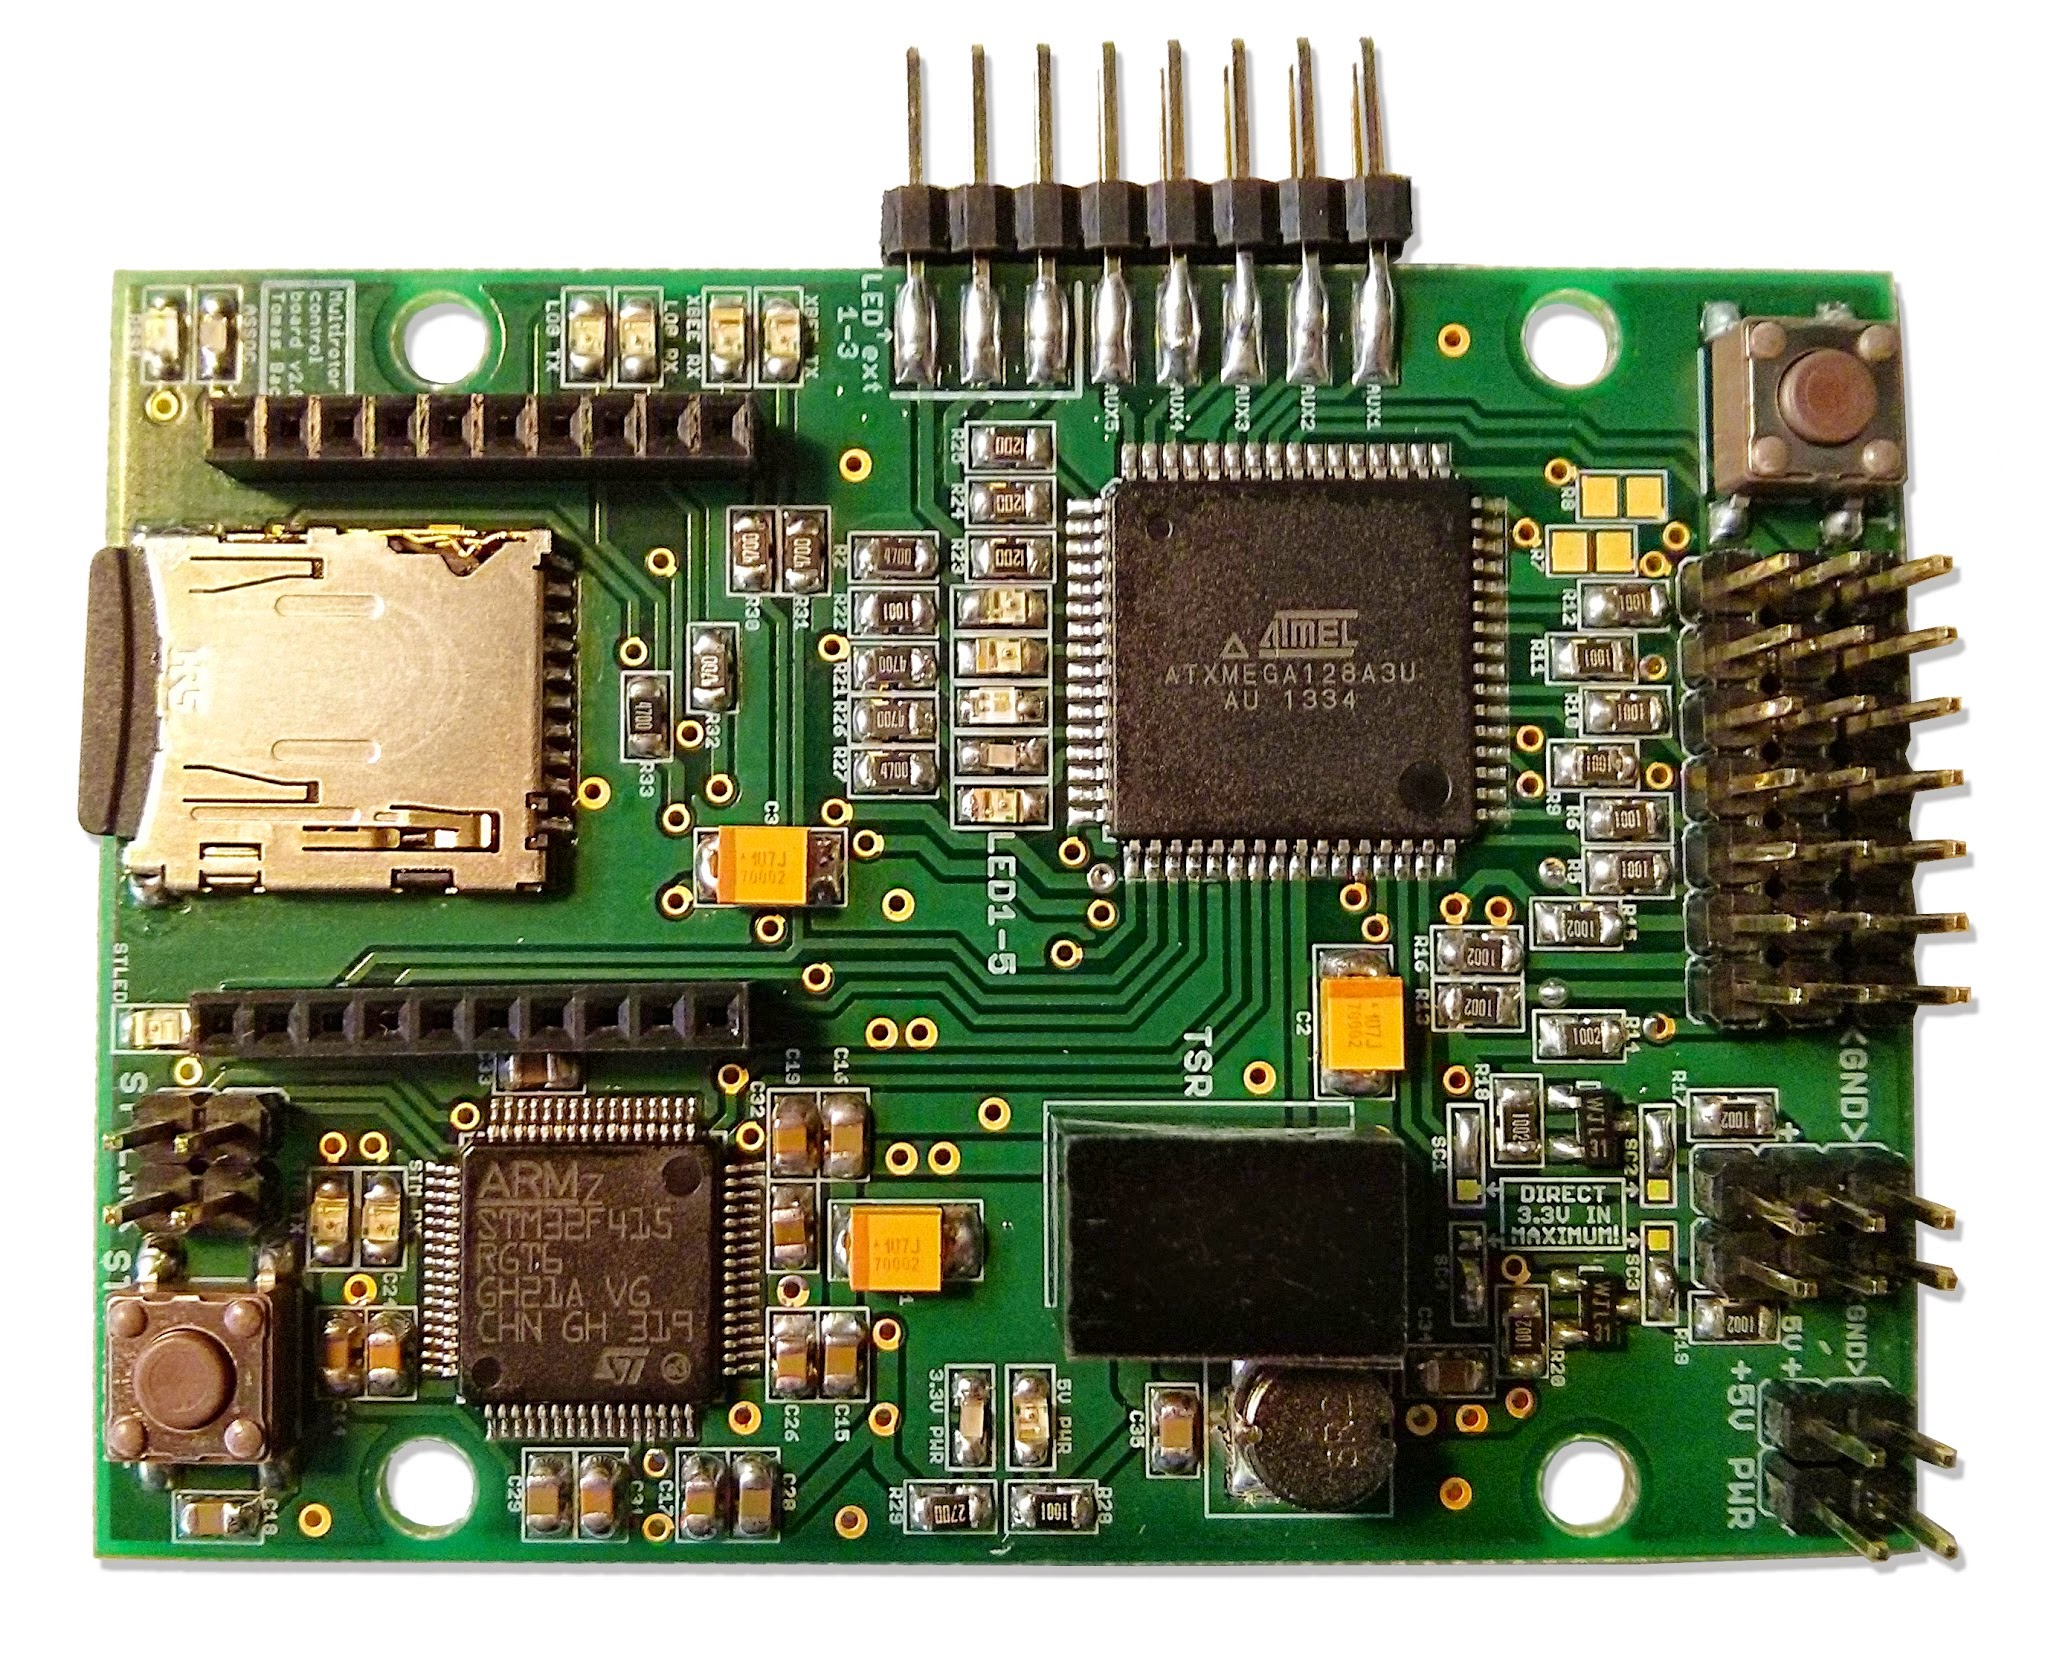
\includegraphics[width=\textwidth]{fig/board1.jpg}
	\caption{Board's top.}
	\label{fig:board_top}
\end{subfigure}%
\begin{subfigure}[b]{0.485\textwidth}
	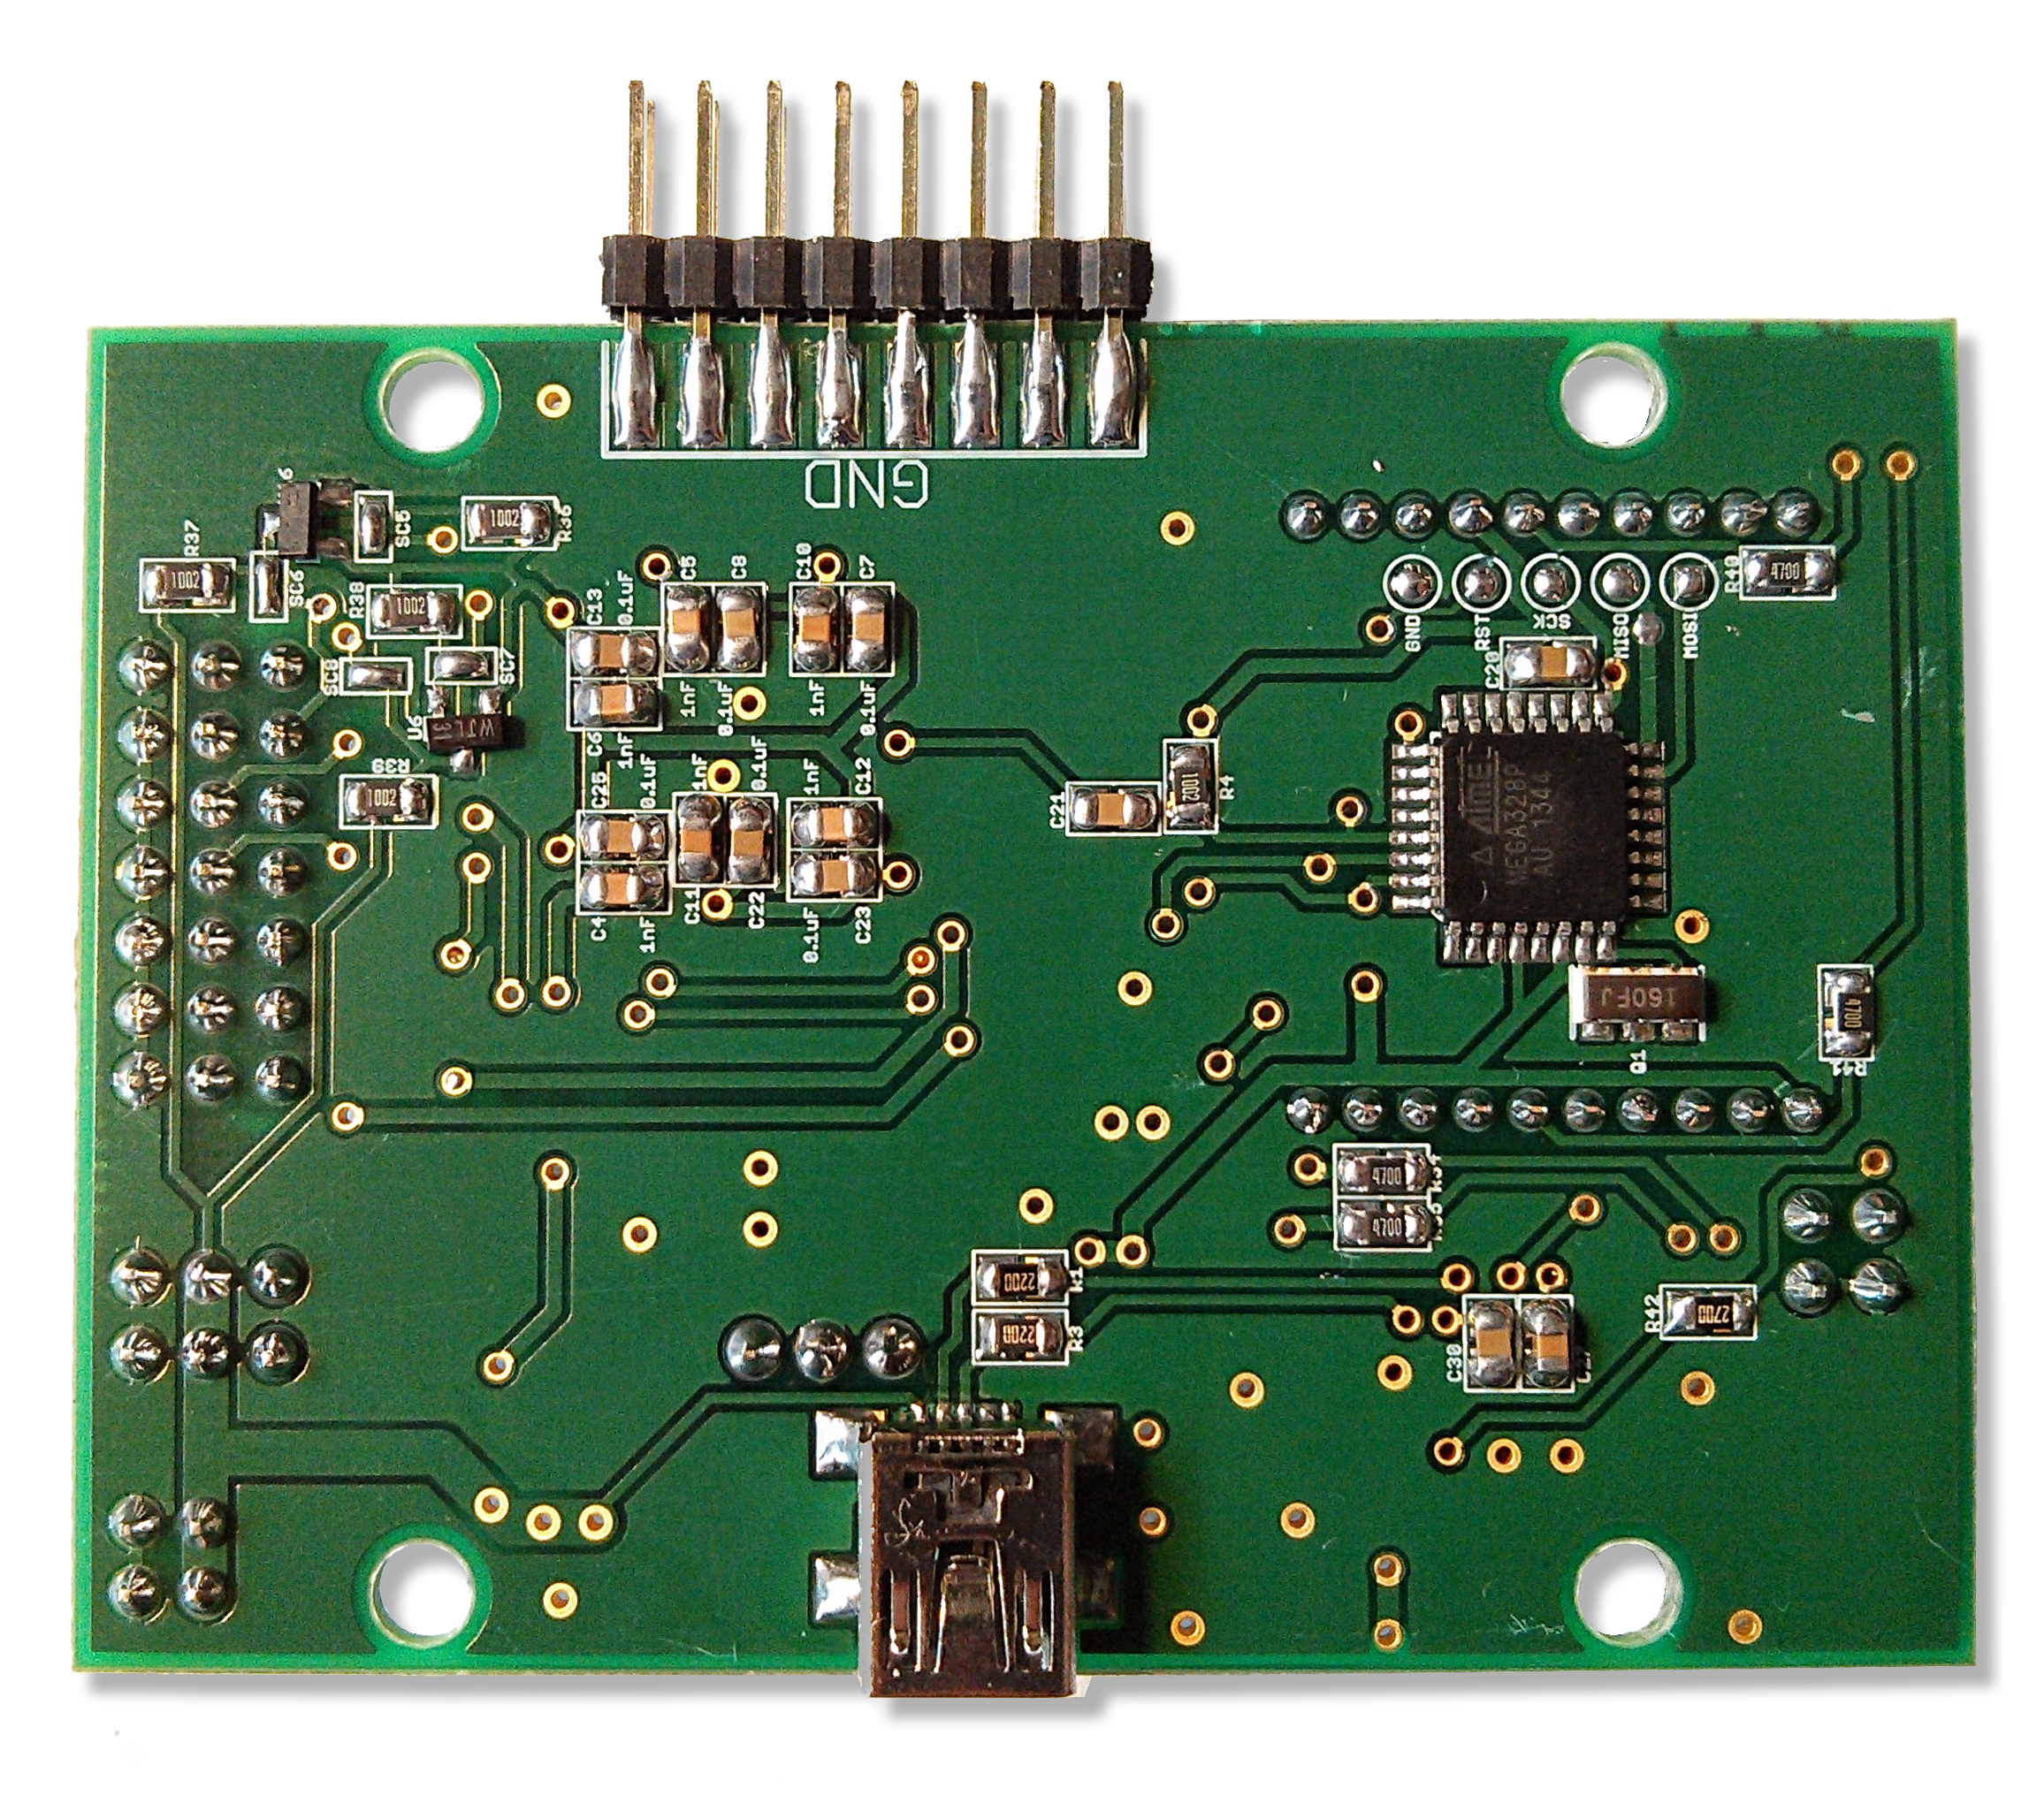
\includegraphics[width=\textwidth]{fig/board2.jpg}
	\caption{Board's bottom.}
	\label{fig:board_bottom}
\end{subfigure}

\caption{Custom control board v.2}
\label{fig:custom_board}
\end{figure}

\subsubsection{xMega main unit}

\subsubsection{ARM co-processing unit}

\subsubsection{XBee telemetry module}

\subsubsection{OpenLog datalogging module}

\subsection{FreeRTOS and tasks}

\subsection{CMatrixLib - ANSI C matrix library}

\subsection{Summary}